\section{Background}
\label{sec:background}

\subsection{Large Language Models}
Modern LLMs are based on transformers.
Transformer models use attention~\cite{vaswani2017attention} and multi-layer-perceptron layers to understand the inputs and generate an output, respectively.
Transformer-based LLMs include encoder-only~\cite{devlin2018bert,liu2019roberta}, decoder-only~\cite{radford2019gpt, scao2022bloom, hf_llama2}, and encoder-decoder~\cite{flan-t5_finetune} models. 
Generative LLMs, the focus of this paper, are usually either decoder-only, or encoder-decoder models.


\subsection{Generative LLM inference phases}
\label{sec:kvcachebg}
\Cref{fig:LLM_example} shows an example of generative LLM inference.
Once the prompt query is received, all the input tokens are computed in parallel, within a single iteration, to generate the first token.
We call this the prompt processing phase.
The context generated from the attention layers during the prompt computation is saved in the key-value (KV) cache, since it is needed for all the future token generation iterations. 
After the first token is generated, the following tokens only use the last generated token and the KV-cache as inputs to the forward pass of the model.
This makes the subsequent token generation more memory bandwidth and capacity intensive than the computationally heavy prompt phase.

%In this paper, we separate the \emph{prompt} and \emph{token} phases of a generative LLM inference on to separate machines.  

\begin{figure}[t]
    \centering
    
\includegraphics[width=1\columnwidth]{figures/query}
    \caption{An LLM inference example.}
    \label{fig:LLM_example}
\end{figure}


\subsection{Performance metrics for LLMs}
Prior work has proposed three main metrics for LLM inference: end-to-end (E2E) latency, time to first token (TTFT), and throughput.
We add another latency metric: time between tokens (TBT), to track the online streaming throughput of the tokens as they are generated serially.
\Cref{tab:perf_metrics} summarizes the key performance metrics that we consider in this work.

\begin{table}[t]
\centering
\footnotesize
\begin{tabular}{@{}ccc@{}}
\toprule
\textbf{Metric}            & \textbf{Importance to user} \\ \midrule
End-to-end (E2E) latency   & Total query time that the user sees        \\
Time to first token (TTFT) & How quickly user sees initial response    \\
Time between tokens (TBT)  & Average token streaming latency           \\
Throughput                 & Requests per second \\ \bottomrule
\end{tabular}
\caption{Performance metrics for LLMs.}
\label{tab:perf_metrics}
\end{table}

Generative LLMs may be used for a variety of tasks with different kinds of SLOs. 
For batch tasks (\eg, summarization), TTFT or TBT latency metrics are less important than throughput.
On the other hand, for latency-sensitive tasks (\eg, conversational APIs), TTFT and TBT are the more important metrics with tighter SLOs.

\begin{figure}[t]
    \centering
    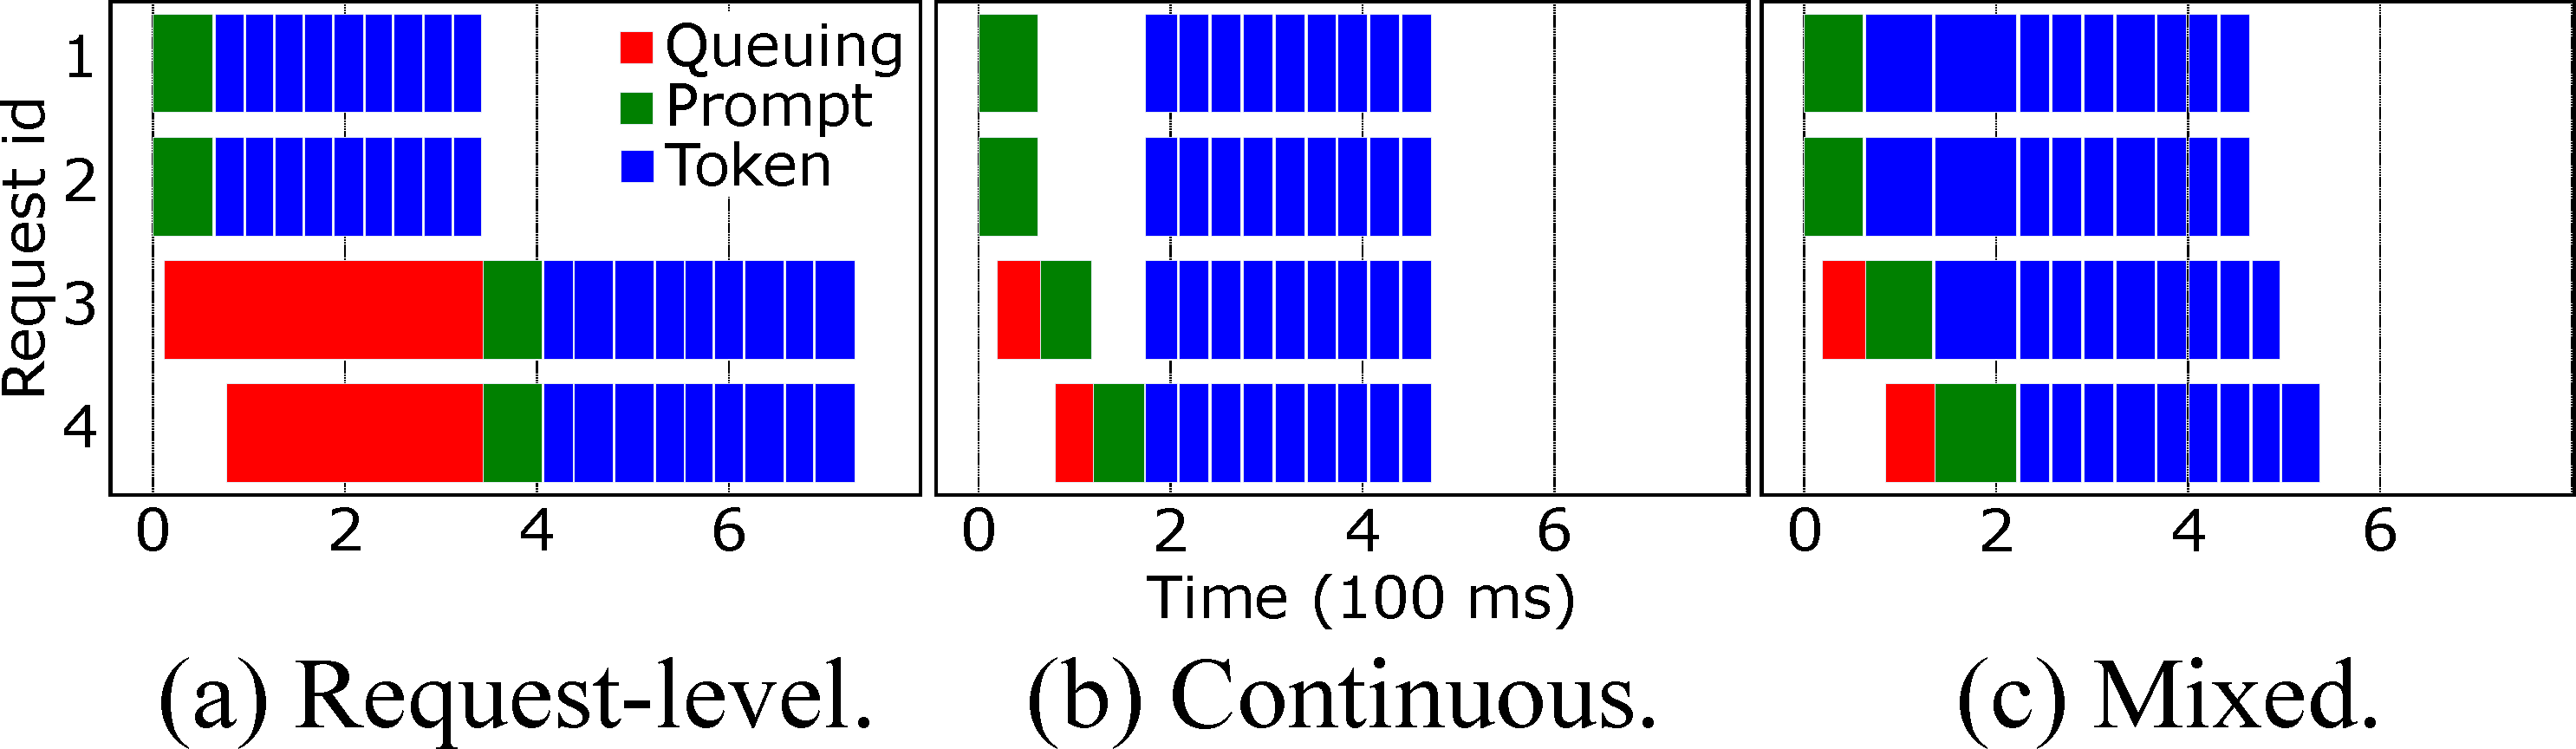
\includegraphics[width=\columnwidth]{figures/characterization/512_batching}
    \caption{Batching mechanisms and their latency impact on the prompt and token phases.
    }
    \label{fig:batching-gantt-chart}
\end{figure}

\subsection{Batching of requests}
Inference requests can be batched together for higher throughput.
Several prior works have explored batching~\cite{yu2022orca,sarathi}.
\Cref{fig:batching-gantt-chart} shows the timelines for inference with three common batching mechanisms.
The default mechanism only batches at the \emph{request-level} (\Cref{fig:batching-gantt-chart}(a)).
In this case, ready requests are batched together, but all the forward passes for these requests are completed before any other requests are run.
Since requests can have long token generation phases, this can lead to long wait times for requests arriving in between, causing high TTFT and high E2E latencies.
An optimization is \emph{continuous batching}~\cite{yu2022orca} (\Cref{fig:batching-gantt-chart}(b)).
In this case, scheduling decisions are made before each forward pass of the model. However, any given batch comprises either only of requests in their prompt phase or only requests in token phase.
Prompt phase is considered more important since it impacts TTFT.
Hence, a waiting prompt can preempt a token phase.
Although this leads to shorter TTFT, it can substantially increase the tail for TBT, and therefore the E2E latency.
Finally, there is \emph{mixed batching} (\Cref{fig:batching-gantt-chart}(c))~\cite{sarathi}.
With this batching, the scheduling decisions are made at each forward pass, and the prompt and token phases can run together.
This reduces the impact on TBT, but does not eliminate it, since token phases scheduled with prompt phases will experience a longer runtime.
In the rest of the paper, we use mixed batching unless stated otherwise.


\subsection{Model parallelism}
\label{sec:modelparallel}
%Given the increasing model sizes, model parallelism is no longer just applicable to training, but also inference.
Model parallelism can be used to divide a model onto multiple GPUs, and even multiple machines, for higher efficiency and memory capacity.
%There are two types of model parallelism used in inference: pipeline and tensor. 
LLM inference typically uses pipeline and tensor parallelism.
Pipeline parallelism (PP) divides the layers of the model among the GPUs, while keeping all the operators and tensors within a layer on the same GPU.
Tensor parallelism (TP) divides the tensor across the GPUs, while replicating all the layers on each GPU.
Pipeline parallelism requires lower communication across the participating GPUs, while tensor parallelism requires high bandwidth communication for each layer. 
In general, tensor parallelism performs better for GPUs within the same machine, connected with high bandwidth interconnects like \eg NVLink~\cite{nvidia_dgx_a100}.
In the rest of the paper, we use tensor parallelism across 8 GPUs for the best latency.


\subsection{GPU clusters and interconnects}
\label{sec:gpu-interconnect}
With the recent rise of LLM use cases, several cloud service providers have expanded the GPU-based offerings, leading to large GPU cluster deployments~\cite{meta_ai_supercluster,azure_openai,coreweave}.
Each machine in these AI clusters is generally comprised of 8 flagship NVIDIA GPUs (A100 or H100).
Each GPU is connected to all the other GPUs in the cluster with a high bandwidth Mellanox InfiniBand interconnect~\cite{infiniband,azure_ib}, forming a high bandwidth data plane network.
The InfiniBand bandwidth offered in the cloud today ranges from 25 to 50GBps per GPU pair~\cite{azure_ib,coreweave_ib}.
%The default optimized communication library across GPUs over NVLink or InfiniBand is NCCL~\cite{nccl}.
